\documentclass{article}
\usepackage[a4paper,margin=1in]{geometry}
\usepackage{amsmath,amsfonts,amssymb,graphicx}
\title{\textbf{CS 370 Winter 2025: Assignment 1}}
\author{Jiaze Xiao \\ 20933691}
\date{\today}
\setlength{\parindent}{0pt}
\begin{document}

\maketitle

\section{Floating Point Basics}
\subsection*{(a)}
Given
$$
    17 = 10001 = 0.10001 \times 2^5.
$$
$$
    17 + 2^{-5} = 10001.00001 = 0.1000100001 \times 2^5.
$$
Thus, $t=10$. Now find the smallest floating-point number larger than 70:
$$
    17 = 1000110 = 0.1000110000 \times 2^7.
$$
As a result, the smallest floating-point number larger than 70 is $\boxed{0.1000110001 \times 2^7}$

\subsection*{(b)}
\begin{itemize}
    \item The smallest positive number is obtained when $d_1 = 1$, $d_2 = d_3 = \cdots = d_t = 0$, and $p = L = -20$:
          $$
              x_{\min} = \boxed{0.1000000000 \times 2^{-20}}.
          $$
    \item The largest positive number is obtained when $d_1 = 1$, $d_2 = d_3 = \cdots = d_t = 1$, and $p = U = 20$:
          $$
              x_{\max} = \boxed{0.1111111111 \times 2^{20}}.
          $$
\end{itemize}

\subsection*{(c)}
$$
    1 = 0.1000000000 \times 2^1
$$
The next representable number:
$$
    1 + 2^{-9} = 0.1000000001 \times 2^1
$$
Thus,
$$
    E = \beta^{1-t} = \boxed{2^{-9}}.
$$

\newpage
\section{Effects of Cancellation}
\subsection*{(a)}
Truncate the given numbers:
$$
    e^{0.1} = 1.105171 = 0.11051 \times 10^1
$$
$$
    e^{-0.1} = 0.904837 = 0.90483 \times 10^0
$$
Then,
\begin{equation*}
    \begin{aligned}
        f(0.1) = & \dfrac{e^{0.1} - e^{-0.1}}{2 \cdot 0.1} \\
        =        & \dfrac{1.1051-0.90483}{0.2}             \\
        =        & \dfrac{0.20027}{0.2}                    \\
        =        & 1.00135                                 \\
        =        & \boxed{0.10013 \times 10^1}
    \end{aligned}
\end{equation*}

\subsection*{(b)}
Substitute Taylor expansions into (1):
$$
    \begin{aligned}
        f(x) = & \dfrac{(1 + x + 0.5x^2 + 0.166x^3 + 0.04166x^4)-(1 - x +0.5x^2 -0.166x^3+0.04166x^4)}{2x} \\
        =      & 0.166 x^2 + 1
    \end{aligned}
$$
Now,
$$
    \begin{aligned}
        f(0.1) = & 0.166 \cdot 0.1^2 + 1       \\
        =        & 0.00166+1                   \\
        =        & \boxed{0.10016 \times 10^1}
    \end{aligned}
$$

\subsection*{(c)}
The original formula in part (a) involves the subtraction of two nearly equal numbers, $e^{0.1}$ and $e^{-0.1}$. This subtraction leads to cancellation error, where the most significant digits are lost, reducing the precision of the result. In part (b), the reformulated expression avoids direct subtraction of nearly equal terms. Thus, the computation in part (b) is more accurate.

\newpage
\section{Floating Point Error Analysis}
\subsection*{The relative error for $(x \otimes x) \ominus 1$}
$$
    \begin{aligned}
        E_{rel}= & \dfrac{|(x \otimes x) \ominus 1 - (x^2 - 1)|}{|x^2 - 1|}                                         \\
        =        & \dfrac{|x^2 (1 + \delta_1) \ominus 1 - (x^2 - 1)|}{|x^2 - 1|}, \quad |\delta_1| \leq E           \\
        =        & \dfrac{|(x^2 (1 + \delta_1) - 1)(1 + \delta_2) - (x^2 - 1)|}{|x^2 - 1|}, \quad |\delta_2| \leq E \\
        =        & \dfrac{|(x^2 - 1)(1 + \delta_2) + x^2 \delta_1(1 + \delta_2) - (x^2 - 1)|}{|x^2 - 1|}            \\
        =        & \dfrac{|\delta_2(x^2 - 1) + x^2 \delta_1(1 + \delta_2)|}{|x^2 - 1|}                              \\
        =        & \dfrac{|(\delta_1+\delta_2+\delta_1\delta_2)x^2 - \delta_2|}{|x^2 - 1|}                          \\
        \leq     & \dfrac{|2Ex^2 - E|}{|x^2 - 1|},\quad\text{ignoring $E^2$}                                        \\
        =        & \boxed{\dfrac{|2x^2 - 1|}{|x^2 - 1|}E}                                                           \\
    \end{aligned}
$$

\subsection*{The relative error for $(x \ominus 1) \otimes (x \oplus 1)$}
$$
    \begin{aligned}
        E_{rel}= & \dfrac{|(x \ominus 1) \otimes (x \oplus 1) - (x^2 - 1)|}{|x^2 - 1|}                                                          \\
        =        & \dfrac{|(x - 1)(1 + \delta_3) \otimes (x \oplus 1) - (x^2 - 1)|}{|x^2 - 1|}, \quad |\delta_3| \leq E                         \\
        =        & \dfrac{|(x - 1)(1 + \delta_3) \otimes (x + 1)(1 + \delta_4) - (x^2 - 1)|}{|x^2 - 1|}, \quad |\delta_4| \leq E                \\
        =        & \dfrac{|\big((x - 1)(1 + \delta_3)(x + 1)(1 + \delta_4)\big)(1 + \delta_5) - (x^2 - 1)|}{|x^2 - 1|}, \quad |\delta_5| \leq E \\
        =        & \dfrac{|(x^2 - 1)(1 + \delta_3)(1 + \delta_4)(1 + \delta_5) - (x^2 - 1)|}{|x^2 - 1|}                                         \\
        \leq     & \dfrac{|(x^2 - 1)(1 + 3E) - (x^2 - 1)|}{|x^2 - 1|}, \quad \text{ignoring higher-order terms of $E^2$}                        \\
        =        & \dfrac{|3E(x^2 - 1)|}{|x^2 - 1|}                                                                                             \\
        =        & \boxed{3E}                                                                                                                   \\
    \end{aligned}
$$

\subsection*{Which of the methods is better?}
The relative error bound for $(x \otimes x) \ominus 1$ is $\frac{|2x^2 - 1|}{|x^2 - 1|}E$, which approximate to $2E$ when $x$ grows. And its smaller than the relative error bound for $(x \ominus 1) \otimes (x \oplus 1)$ of $3E$, indicating $(x \otimes x) \ominus 1$ is better. However, when $x$ is small (especially close to 1), cancellation errors will make the computation of $(x \otimes x) \ominus 1$ unstable. As a result,
\begin{itemize}
    \item For large $x$, $(x \otimes x) \ominus 1$ is better.
    \item For $x\approx 1$, $(x \ominus 1) \otimes (x \oplus 1)$ is better.
\end{itemize}


\newpage
\section{Polynomial Interpolation}
To solve the cubic polynomial $p(x) = ax^3 + bx^2 + cx + d$, apply the given conditions.
\begin{itemize}
    \item Condition $ p(0) = 1 $:
          $$
              p(0) = a(0)^3 + b(0)^2 + c(0) + d = d = 1
          $$
          So, $ d = 1 $.
    \item Condition $ p'(0) = v $:\\
          The derivative of $ p(x) $ is:
          $$
              p'(x) = 3ax^2 + 2bx + c
          $$
          At $ x = 0 $:
          $$
              p'(0) = 3a(0)^2 + 2b(0) + c = c
          $$
          So, $ c = v $.
    \item Condition $ p'(1) = v + 6u $:
          $$
              p'(1) = 3a(1)^2 + 2b(1) + c = 3a + 2b + c
          $$
          Substituting $ c = v $:
          $$
              3a + 2b + v = v + 6u
          $$
          Simplify:
          \begin{equation*}
              3a + 2b = 6u \tag{1}
          \end{equation*}
    \item Condition $ p''(1) = 8u $:\\
          The second derivative of $ p(x) $ is:
          $$
              p''(x) = 6ax + 2b
          $$
          At $ x = 1 $:
          $$
              p''(1) = 6a(1) + 2b = 6a + 2b
          $$
          Given $ p''(1) = 8u $:
          \begin{equation*}
              6a + 2b = 8u \tag{2}
          \end{equation*}
\end{itemize}

Subtract equation (1) from equation (2):
$$
    \begin{aligned}
        (6a + 2b) - (3a + 2b) = & 8u - 6u      \\
        3a =                    & 2u           \\
        a =                     & \frac{2u}{3}
    \end{aligned}
$$
Substitute $ a = \frac{2u}{3} $ into equation (1):
$$
    \begin{aligned}
        3\left(\frac{2u}{3}\right) + 2b = & 6u \\
        2u + 2b =                         & 6u \\
        b =                               & 2u
    \end{aligned}
$$
Thus, the cubic polynomial is:
$$
    \boxed{p(x) = \frac{2u}{3}x^3 + 2ux^2 + vx + 1}
$$

\newpage
\section{Spline Construction}
\subsection*{(a)}
Given points:
$$
    x = [-2, 0, 1, 3, 6], \quad y = [2, -1, -1, 3, 2].
$$
Step sizes ($\Delta x$):
$$
    \Delta x_1 = 2, \quad \Delta x_2 = 1, \quad \Delta x_3 = 2, \quad \Delta x_4 = 3.
$$

Slopes ($y'_i$) between points:
$$
    y'_1 = \frac{y_2 - y_1}{x_2 - x_1} = \frac{-1 - 2}{0 - (-2)} = -\frac{3}{2},
$$
$$
    y'_2 = \frac{y_3 - y_2}{x_3 - x_2} = \frac{-1 - (-1)}{1 - 0} = 0,
$$
$$
    y'_3 = \frac{y_4 - y_3}{x_4 - x_3} = \frac{3 - (-1)}{3 - 1} = 2,
$$
$$
    y'_4 = \frac{y_5 - y_4}{x_5 - x_4} = \frac{2 - 3}{6 - 3} = -\frac{1}{3}.
$$

From the general form of $T$:
$$
    T_{i, i-1} = \Delta x_{i-1}, \quad T_{i, i} = 2(\Delta x_{i-1} + \Delta x_i), \quad T_{i, i+1} = \Delta x_i \quad \text{for }i=2,\dots,n-1
$$
and having clamped boundary conditions at both
ends, we construct $T$ as:
$$
    T =
    \begin{bmatrix}
        1 & 0 & 0 & 0  & 0 \\
        2 & 6 & 1 & 0  & 0 \\
        0 & 1 & 6 & 2  & 0 \\
        0 & 0 & 2 & 10 & 3 \\
        0 & 0 & 0 & 0  & 1
    \end{bmatrix}.
$$

For $i = 2, \dots, n-1$, $r_i = 3(\Delta x_i y'_{i-1} + \Delta x_{i-1} y'_i)$:
$$
    r_2 = 3(\Delta x_2 y'_1 + \Delta x_1 y'_2) = 3(1 \cdot (-\frac{3}{2}) + 2 \cdot 0) = -\frac{9}{2},
$$
$$
    r_3 = 3(\Delta x_3 y'_2 + \Delta x_2 y'_3) = 3(2 \cdot 0 + 1 \cdot 2) = 6,
$$
$$
    r_4 = 3(\Delta x_4 y'_3 + \Delta x_3 y'_4) = 3(3 \cdot 2 + 2 \cdot (-\frac{1}{3})) = 3(6 - \frac{2}{3}) = 16.
$$

Boundary conditions modify:
$$
    r_1 = 1, \quad r_5 = 1.
$$

Thus:
$$
    \vec{r} = \begin{bmatrix}
        1            \\
        -\frac{9}{2} \\
        6            \\
        16 \\
        1
    \end{bmatrix}.
$$

As a result, here is the final linear system:
$$
    T \vec{s} = \vec{r}, \quad
    T =
    \begin{bmatrix}
        1 & 0 & 0 & 0  & 0 \\
        1 & 6 & 2 & 0  & 0 \\
        0 & 2 & 6 & 1  & 0 \\
        0 & 0 & 3 & 10 & 2 \\
        0 & 0 & 0 & 0  & 1
    \end{bmatrix}, \quad
    \vec{r} =
    \begin{bmatrix}
        1            \\
        -\frac{9}{2} \\
        6            \\
        16 \\
        1
    \end{bmatrix}.
$$

\subsection*{(b)}
After solving the linear equation, we get:
$$
    \vec{s} =
    \begin{bmatrix}
        1          \\
        -1.34271523\\
        1.2781457\\
        1.01655629\\
        1
    \end{bmatrix}.
$$
According to $c_i=\dfrac{3y'_i-2s_i-s_{i+1}}{\Delta x_i}$ and $d_i=\dfrac{s_{i+1}+s_i-y'_i}{(\Delta x_i)^2}$, now we have:
$$
    a_1=2, a_2=-1, a_3=-1, a_4=3
$$
$$
    b_1=1, b_2=-1.343, b_3=1.278, b_4=1.017
$$
$$
    c_1=-2.579, c_2=1.407, c_3=1.214, c_4=-1.344
$$
$$
    d_1=0.6643, d_2=-0.06457, d_3=-0.4263, d_4=0.2981
$$
(Process included in \texttt{A1Q5.ipynb})

\subsection*{(c)}
\begin{center}
    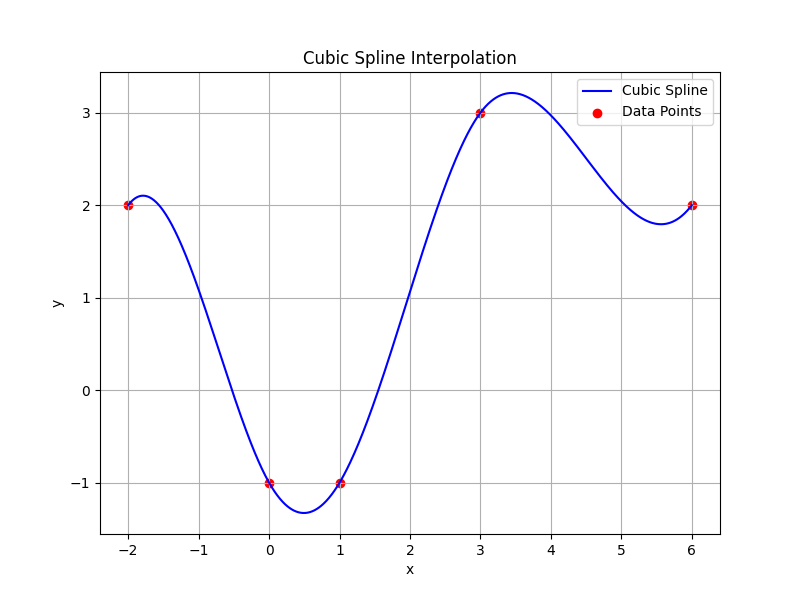
\includegraphics[scale=0.78, keepaspectratio]{q5c.png}
\end{center}
(Process included in \texttt{A1Q5.ipynb})

\end{document}
